\documentclass[12pt]{article}

\usepackage{graphicx}
\usepackage{amsmath}
\usepackage{amssymb}
\usepackage{natbib}
\usepackage{amsfonts}
\usepackage{multicol}
\usepackage{float}
\usepackage{oldgerm}
\usepackage{bm}
\usepackage{mathtools}
\usepackage{wrapfig}
\usepackage{fancyhdr}
\usepackage[export]{adjustbox}
\usepackage{xcolor}
\usepackage[shortlabels]{enumitem}

\pagestyle{empty}

\setlength{\headsep}{0.5cm}
\setlength{\oddsidemargin}{-0.5cm}
\setlength{\textwidth}{16.5cm}
\setlength{\textheight}{24cm}
\voffset = -2cm


\pagestyle{fancy}
\fancyhf{}
\rfoot{
\includegraphics[width=1.0in]{cnm.png}}
\lfoot{Homework 9}
\setlength\parindent{0pt}
\begin{document}

\begin{center}
\hfil
{\large\bf {ENGR 2910-101: Circuit Analysis}}
\hfill Instructor: Brian Rashap\\
Homework 9: \hfill Due: See Brightspace\\
\hrulefill\\
\end{center}

{\bf Question 1} [5] % P8-02

For the circuit below, $R = 200 \Omega$, $L = 50 mH$, $C=0.2\mu F$. The initial inductor current is $-45mA$ and the initial capacitor voltage is $15V$. 

\begin{figure}[h!]
\begin{center}
 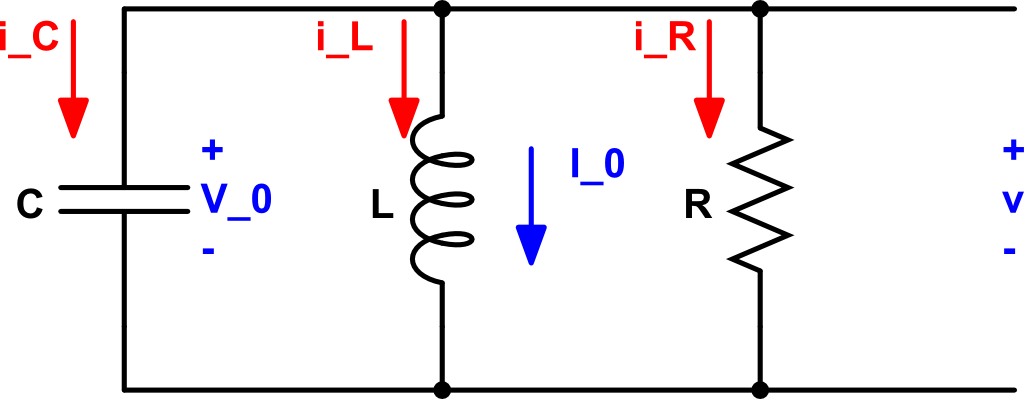
\includegraphics[scale=0.4]{fig8_1.png}
\end{center}
\end{figure}

\begin{enumerate}[(a)]
\item Calculate the initial current for each branch of the circuit.
\item Find $v(t)$ for $t \geq 0$.
\item Find $i_L(t)$ for $ \geq 0$.
\end{enumerate}


\vspace{0.1in}


{\bf Question 2} [5] % P8-32

For the circuit below with $R = 12.5 \Omega$, $L = 25 mH$, $C=62.5\mu F$. Assume that at the instant that the 2A current source is applied to the circuit, the initial inductor current is $1A$ and that the initial capacitor voltage is $50 V$.
Find the expression for $i_L(t)$ for $t \geq 0$. 

\begin{figure}[h!]
\begin{center}
 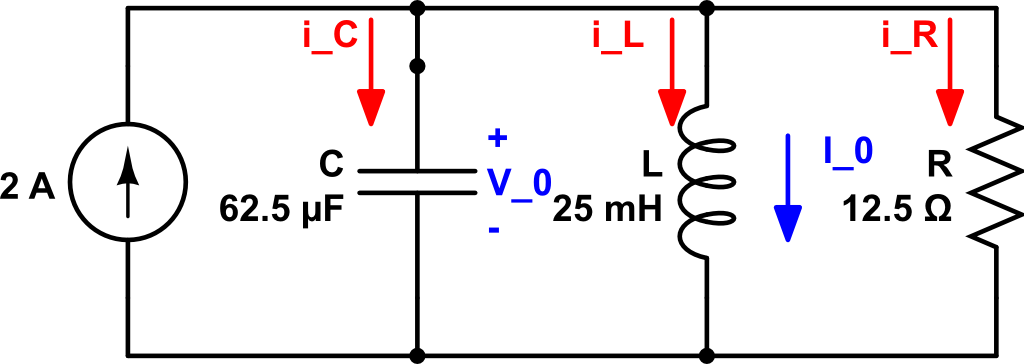
\includegraphics[scale=0.6]{fig8_32.png}
\end{center}
\end{figure}

\newpage

{\bf Question 3} [5] % P8-41

The current in the circuit below is known to be
\begin{equation}
i(t) = B_1 e^{-2000t} \cos{(1500t)} + B_2 e^{-2000t} \sin{(1500t)}, t \geq 0 
\end{equation}
\begin{figure}[h!]
\begin{center}
 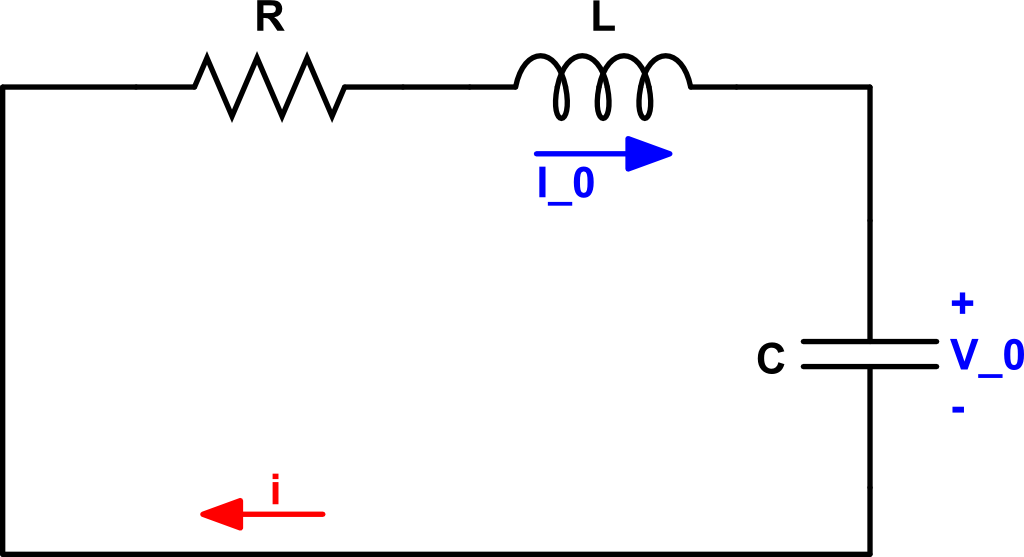
\includegraphics[scale=0.4]{fig8_3.png}
\end{center}
\end{figure}

The capacitor has a value of $80 nF$, the initial current is $7.5mA$, and the initial voltage across the capacitor is $-30V$. Find $R, L, B_1, B_2$.

\vspace{0.5cm}

{\bf Question 4 [5]} % P8_46

The switch in the circuit below has been at Position A for a long time. At $ t = 0$, the switch is moved instantaneously to Position B. 

\begin{figure}[h!]
\begin{center}
 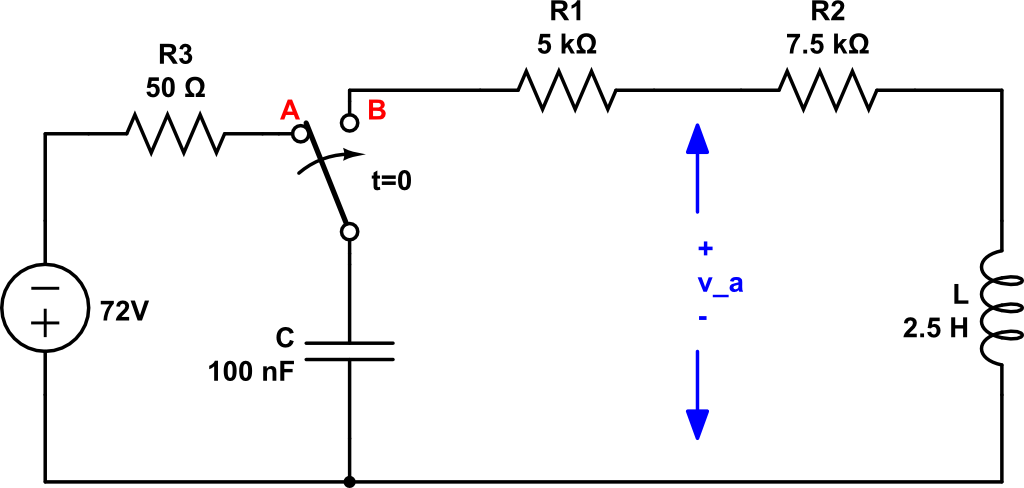
\includegraphics[scale=0.6]{fig8_46.png}
\end{center}
\end{figure}

\begin{enumerate}[(a)]
\item What is the initial value for $v_a$?
\item What is the initial value for $\frac{dv_a}{dt}$?
\item What is the numerical expression for $v_a(t)$ for $t \geq 0$.
\end{enumerate}

\end{document}
